\documentclass[aspectratio=169]{beamer}

\usepackage[utf8]{inputenc}

\usepackage{amsfonts}
\usepackage{amsmath}
\usepackage{color}
\usepackage{listings}
\usepackage{tikz}
\usepackage{hyperref}

\usetheme{Rochester}
\usecolortheme{beaver}

\addtobeamertemplate{navigation symbols}{}{%
    \usebeamerfont{footline}%
    \usebeamercolor[fg]{footline}%
    \hspace{1em}%
    \insertframenumber/\inserttotalframenumber
}

\lstloadlanguages{C++}
    \lstset{%
        language={C++},
        basicstyle=\ttfamily,
        keywordstyle=\color{blue},
        showstringspaces=false,
        escapechar={§},
        escapeinside=||
    }

\newif\iftransitions
 \transitionstrue


\newif\iffast
% \fasttrue

\title{Exceptions Demystified}
% \subtitle{An Introduction to Custom Allocators}
\author{Andreas Weis}
\institute{BMW AG}

\date{MUC++, April 25, 2019}
%\titlegraphic{
\includegraphics[height=.15\textheight]{resources/accu2019_logo.png}}

\iffalse
Exceptions Demystified

Exception Handling is probably one of the most controversial features in C++, with many code bases outright banning them from the start, or only allowing their use in very specific cases. The reasons for this are often unclear and founded on premises that are not well understood.

In this talk, we will explain exception handling from the bottom up, taking a close look at what a compiler actually has to do to implement the mechanism. Instead of focusing on a specific implementation, we will approach the problem from a more abstract, language-design point of view, allowing us to explore the different approaches an implementation could choose. In the end, we will gain a deeper understanding for the problems associated with the feature and how they could be mitigated in the future by alternative language features like the proposed static exceptions.


Audience
Language users familiar with exceptions, but not with the underlying implementation

Outline
- Lifetime of an exception
- Anatomy of the call stack
- Finding the right catch
- RTTI
- Unwinding the stack
- Exceptions in restricted environments (real-time, embedded)
- Execution time analysis in the presence of exceptions
- Alternative mechanisms (static exceptions)

Video
https://www.youtube.com/watch?v=S7I66lZX_zM
https://www.youtube.com/watch?v=FcpmMmyNNv8
https://www.youtube.com/watch?v=_8vMAkCp0Rc

Comments
This talk is similar in spirit to Dave Watson's CppCon 2017 talk (https://www.youtube.com/watch?v=_Ivd3qzgT7U) or James McNellis' CppCon 2018 talk (https://www.youtube.com/watch?v=COEv2kq_Ht8). Unlike those, I don't want to focus on a specific implementation, but explain the underlying algorithmic problems that these implementations want to solve. The focus here will also be very much on how those influence the life of an application developer and hopefully separate the valid concerns about exceptions as a feature from the FUD.
\fi

\begin{document}

\frame{\titlepage}

\iftrue %crop

\begin{frame}[fragile]
  \frametitle{About me}

  \begin{itemize}
    \setlength\itemsep{1.5em}

    \item \href{https://stackoverflow.com/users/577603/comicsansms}{
\includegraphics[height=.05\textheight]{resources/so-icon.png}} \href{https://github.com/ComicSansMS}{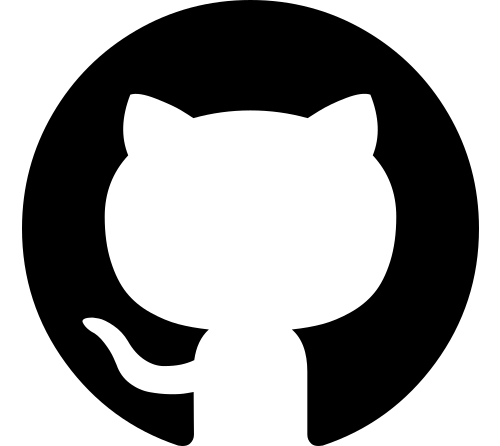
\includegraphics[height=.05\textheight]{resources/github-icon.png}} 
\includegraphics[height=.05\textheight]{resources/slack-icon.png} ComicSansMS

    \item \href{https://twitter.com/DerGhulbus/}{
\includegraphics[height=.05\textheight]{resources/twitter-icon.png} @DerGhulbus}

    \item 
\includegraphics[height=.05\textheight]{resources/meetup-icon.png} Co-organizer of the \href{https://www.meetup.com/MUCplusplus/}{Munich C++ User Group}

    \item Currently working as a Software Architect for BMW 
\includegraphics[height=.1\textheight]{resources/bmw_group.jpg}

  \end{itemize}
\end{frame}


\begin{frame}
  \frametitle{Overview}
  \begin{itemize}
  \item Implementing Exception Handling
  \item Dealing with the problems today
  \item Alternative mechanisms (static exceptions)
  \end{itemize}
\end{frame}


\begin{frame}
  \frametitle{The goal}

  \begin{center}
    Make exceptions usable for everyone.
  \end{center}
\end{frame}

\begin{frame}
  \frametitle{Anatomy of the call stack}

  \begin{columns}
    \begin{column}{.5\textwidth}
      \includegraphics<1-2>[height=.95\textheight]{excgfx/stack_010.png}
      \includegraphics<3>[height=.95\textheight]{excgfx/stack_020.png}
      \includegraphics<4>[height=.95\textheight]{excgfx/stack_030.png}
      \includegraphics<5>[height=.95\textheight]{excgfx/stack_040.png}
      \includegraphics<6>[height=.95\textheight]{excgfx/stack_050.png}
      \includegraphics<7>[height=.95\textheight]{excgfx/stack_060.png}
      \includegraphics<8>[height=.95\textheight]{excgfx/stack_070.png}
      \includegraphics<9>[height=.95\textheight]{excgfx/stack_080.png}
      \includegraphics<10>[height=.95\textheight]{excgfx/stack_090.png}
    \end{column}

    \begin{column}{.5\textwidth}
      \begin{semiverbatim}
        \uncover<2->{f();}  \uncover<2-4>{{\color{green}<= IP}}

        \uncover<5->{{\color{blue}void} f() \{}

        \uncover<5->{\hspace{20pt}{\color{blue}int} x, y, z;}

        \uncover<5->{\hspace{20pt}g();} \uncover<5-8>{{\color{green}<= IP}}

        \uncover<5->{\}}

        \uncover<9->{{\color{blue}void} g() \{}

        \uncover<9->{\hspace{20pt}{\color{blue}int} x;} \uncover<9>{{\color{green}<= IP}}

        \uncover<10->{\hspace{20pt}h();} \uncover<10->{{\color{green}<= IP}}

        \uncover<9->{\}}
      \end{semiverbatim}
    \end{column}
  \end{columns}

\end{frame}

\begin{frame}
  \frametitle{A few observations\ldots}

  \begin{columns}
    \begin{column}{.5\textwidth}
      \includegraphics<1>[height=.95\textheight]{excgfx/stack_090.png}
    \end{column}

    \begin{column}{.5\textwidth}
      \begin{itemize}
      \item The state of the current function is always located between the frame pointer and the stack pointer.
      \item The stack frames form a singly linked that can be traversed by following the frame pointer
        \item When the size of the frame is static, the compiler may generate code that does not rely on the frame pointer to free up a register.
      \end{itemize}
    \end{column}
  \end{columns}
\end{frame}


\begin{frame}[fragile]
  \frametitle{Lifetime of an exception}
  \begin{lstlisting}[language={C++}]
void g() {
    throw MyException{};  // starts here
}

void f() {
  try {
    g();
  } catch(MyException& e) {
  } // dies here
}
  \end{lstlisting}
\end{frame}


\begin{frame}
  \frametitle{Responsibilities of \texttt{throw}}

  \begin{itemize}
  \item Create the exception object
    \begin{itemize}
    \item Memory for the exception is allocated in an unspecified way [except.throw]
    \item As a consequence, there is no official customization point for this allocation
    \item Many implementations today simply perform a heap allocation (even for a single \texttt{int})
    \end{itemize}
  \item Transfer control to the exception handler
    \begin{itemize}
    \item The standard does not mention how this transfer of control is achieved
    \item It does mandate though, that destructors must be invoked for objects along the path from \texttt{throw} to the handler $\Rightarrow$ \emph{stack unwinding} [except.ctor]
    \end{itemize}
  \end{itemize}
\end{frame}


\begin{frame}[fragile]
  \frametitle{Lifetime of an exception}
  \begin{lstlisting}[language={C++}]
void g() {
    throw MyException{};
}

void f() {
  try {
    g();
  } catch(MyException& e1) {
    try {
      g();
    } catch(MyException& e2) {
      // e1 and e2 are both alive in here
    }
  }
}
  \end{lstlisting}
\end{frame}

\begin{frame}[fragile]
  \frametitle{Lifetime of an exception}
  \begin{lstlisting}[language={C++}]
void g() {
    throw MyException{};
}

std::exception_ptr g_exc;

void f() {
  try {
    g();
  } catch(...) {
    g_exc = std::current_exception();
  }
}
  \end{lstlisting}
\end{frame}

\begin{frame}[fragile]
  \frametitle{Lifetime of an exception}
  \begin{lstlisting}[language={C++}]
void g() {
    throw MyException{};
}

std::vector<std::exception_ptr> g_excs;

void f() {
  try {
    g();
  } catch(...) {
    g_excs.push_back(std::current_exception());
  }
}
  \end{lstlisting}
\end{frame}


\begin{frame}
  \frametitle{Storage of the exception object}

  \begin{itemize}
  \item An unbounded number of exception objects can be alive at the same time
  \item Exception objects can be of arbitrary size. Allocate on the heap?
  \item \texttt{std::bad\_alloc} is a common exception
  \item Stack?
  \item We still need to perform calls to destructors during unwinding (each of which can have their own, nested exceptions)
  \item Since C++11, an exception can outlive the handler (\texttt{exception\_ptr}), so these for sure cannot be left on the stack
  \end{itemize}
\end{frame}

\begin{frame}
  \frametitle{Customizing storage of the exception object}
  \begin{itemize}
  \item Most implementations today simply invoke malloc for allocating storage for the exception object
  \item Replacing malloc can be an option for certain scenarios, requires patching the runtime
  \item Is it a problem to allocate exceptions from a fixed-size arena? It might be, as that turns each \texttt{throw} and \texttt{exception\_ptr} use into a potential \texttt{terminate}
  \item In practice, we already have a similar situation today with \texttt{bad\_alloc}
  \end{itemize}
\end{frame}


\begin{frame}
  \frametitle{Responsibilities of \texttt{throw}}

  \begin{itemize}
  \item {\color{gray}Create the exception object}
    \begin{itemize}
    \item {\color{gray}Memory for the exception is allocated in an unspecified way [except.throw]}
    \item {\color{gray}As a consequence, there is no official customization point for this allocation}
    \item {\color{gray}Many implementations today simply perform a heap allocation (even for a single \texttt{int})}
    \end{itemize}
  \item Transfer control to the exception handler
    \begin{itemize}
    \item The standard does not mention how this transfer of control is achieved
    \item It does mandate though, that destructors must be invoked for objects along the path from \texttt{throw} to the handler $\Rightarrow$ \emph{stack unwinding} [except.ctor]
    \end{itemize}
  \end{itemize}
\end{frame}


\begin{frame}
  \frametitle{Finding the right \texttt{catch}}

    \begin{columns}
    \begin{column}{.5\textwidth}
      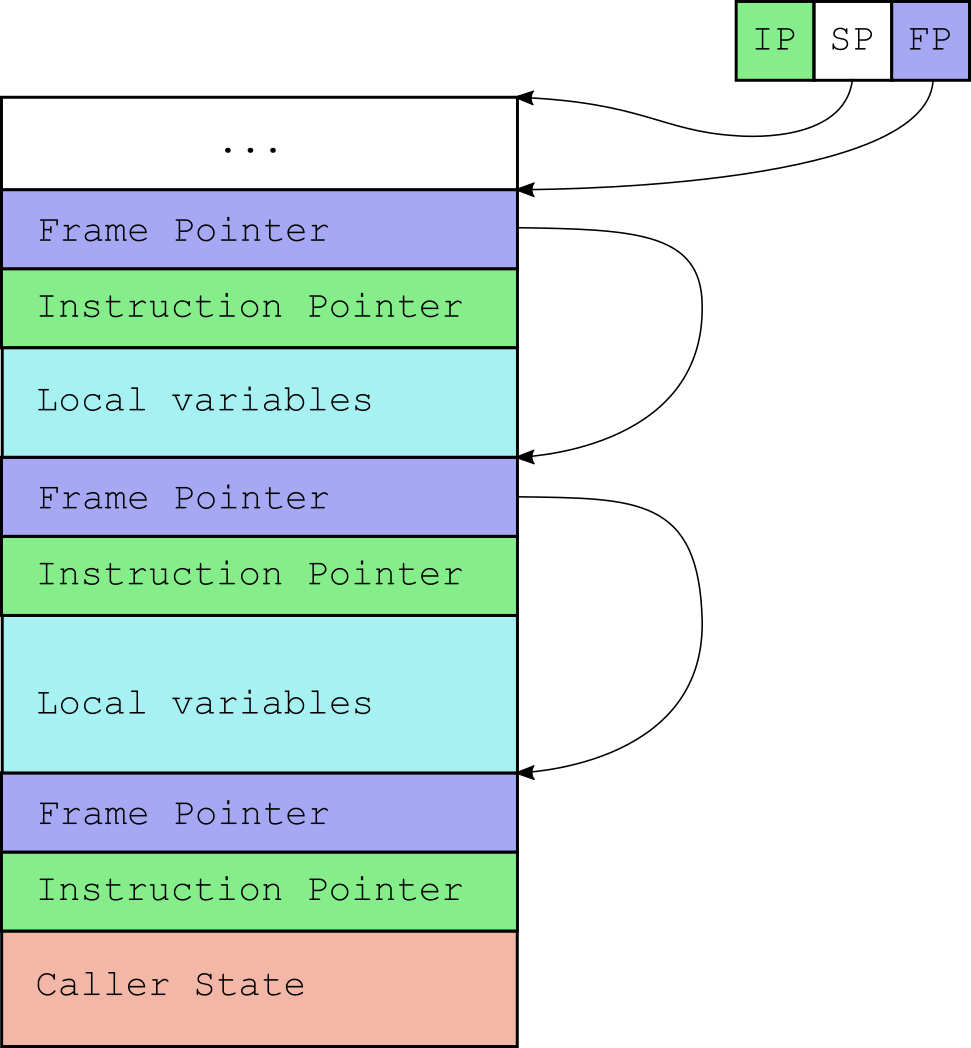
\includegraphics[height=.95\textheight]{excgfx/stack_090.png}
    \end{column}

    \begin{column}{.5\textwidth}
      \begin{itemize}
      \item The stack frames form a linked list that can be iterated over
      \item Traverse the call stack up and check at each level if a matching catch handler is present
      \item Once a catch handler has been found, transfer control to that stack frame
      \end{itemize}
    \end{column}
  \end{columns}
\end{frame}


\begin{frame}[fragile]
  \frametitle{What's the \texttt{catch}?}

  \begin{lstlisting}[language={C++}]
class MyException : public std::exception { /* ... */ };

void g() {
  throw MyException{};
}

void f() {
  try {
    g();
  } catch(std::exception& e) {
    printError(e.what());
  }
}
  \end{lstlisting}
\end{frame}


\begin{frame}
  \frametitle{Finding the right \texttt{catch}}

  \begin{itemize}
  \item Exception types are not required to match exactly
  \item Polymorphic catching of exceptions requires determining the types of all base classes of an object at runtime
  \item Exception class hierarchies are typically complex (one of the few places where multiple inheritance is still common)
  \item There exists a solution for this problem in C++ already: RTTI
  \end{itemize}
\end{frame}


\begin{frame}[fragile]
  \frametitle{Runtime Type Identification (RTTI)}

  \begin{lstlisting}[language={C++}]
class MyException : public std::exception { /* ... */ };

MyException e;
  \end{lstlisting}

  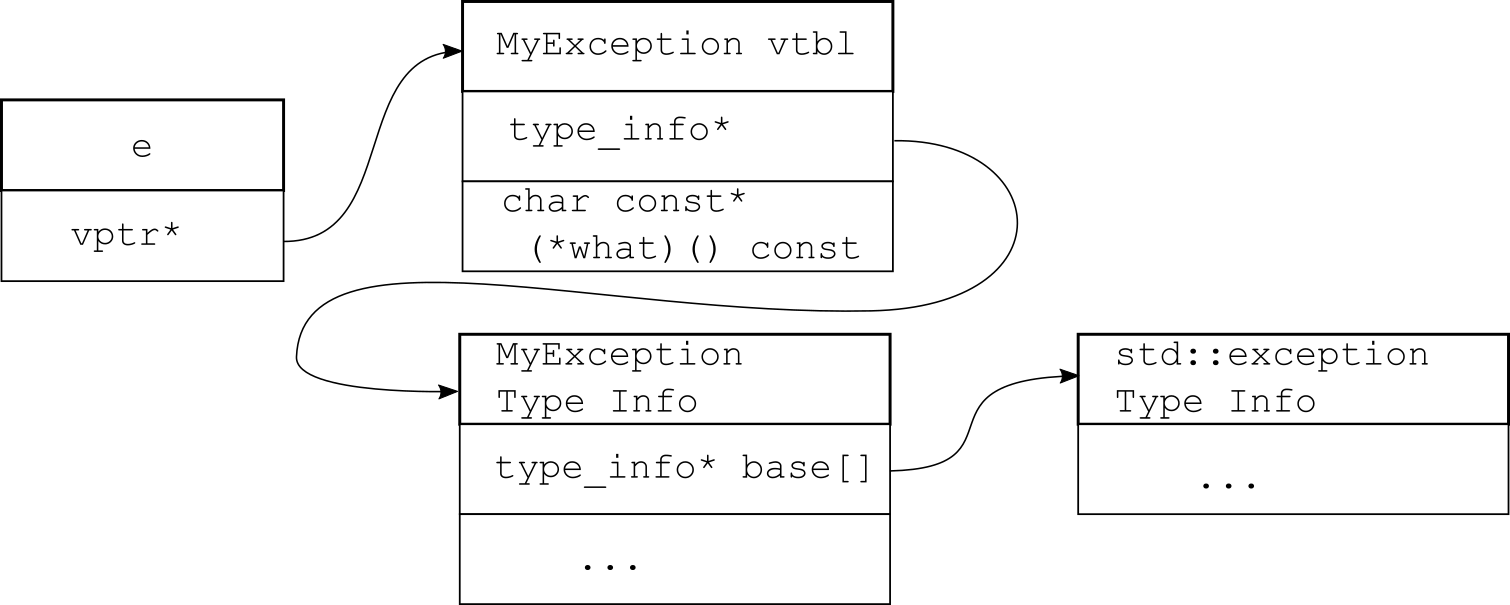
\includegraphics[width=.8\textwidth]{excgfx/rtti_010.png}
\end{frame}


\begin{frame}

  \frametitle{Problems with RTTI}

  \begin{itemize}
  \item Traversing the Type Info structure is expensive
  \item The type info structures are open for extension - pulling in a shared library can increase cost of traversals in existing code
  \item Runtime analysis only possible if all types are known beforehand
  \item RTTI always brings a non-zero overhead for the binary size:
    \begin{itemize}
    \item Type information is stored for all types, not just the ones participating in exception handling
    \item The type info structure contains more information than is needed to find the matching catch handler
    \end{itemize}
  \end{itemize}

  An implementation is not required to use RTTI for exception handling. But they typically do.
\end{frame}


\begin{frame}
  \frametitle{Unwinding the stack}

  
\includegraphics[height=.15\textheight]{excgfx/registers.png}

  \vspace{24pt}

  The state of the program at any point is determined by
  \begin{itemize}
  \item The contents of its memory
  \item The values stored in its registers
  \end{itemize}
\end{frame}

\begin{frame}
  \frametitle{Unwinding the stack}

  \begin{columns}
    \begin{column}{.5\textwidth}
      \includegraphics<1>[height=.95\textheight]{excgfx/stack_090.png}
      \includegraphics<2>[height=.95\textheight]{excgfx/stack_unwind_010.png}
      \includegraphics<3->[height=.95\textheight]{excgfx/stack_unwind_020.png}
    \end{column}

    \begin{column}{.5\textwidth}
      \begin{semiverbatim}
        \alert<1>{IP = old\_IP;}

        \alert<1>{SP = old\_SP;}

        \alert<1>{FP = old\_FP;}
      \end{semiverbatim}
      \uncover<4>{Any problems with this solution?}
    \end{column}
  \end{columns}
\end{frame}


\begin{frame}
  \frametitle{What about destructors?}

  Frame-based Exception Handling

  \begin{itemize}
  \item The program code actively maintains a dynamic data structure for unwinding
  \item Has to keep track of active objects with non-trivial destructors and any enclosing exception handlers
  \item Compiler inserts code to update these data structures accordingly while stepping through the code
  \end{itemize}

  Drawbacks of this approach:
  \begin{itemize}
  \item Maintaining the data structure is costly and has to be done even if no exception ever occurs
  \item Binary code size increases significantly
  \end{itemize}
\end{frame}


\begin{frame}
  \frametitle{What about destructors?}

  Table-based Exception Handling

  \begin{itemize}
  \item The set of active local objects at a certain point in code is known at compile time
  \item Compiler generates a table from code locations to active objects
  \item During unwinding, for each stack frame use the IP as a key for a lookup into the table
  \item If no exception occurs, no additional code for error handling is executed (zero-overhead exceptions)
  \end{itemize}

  Drawbacks of this approach:
  \begin{itemize}
  \item Binary size increases even more to store tables
  \item Table lookup for executing exceptions is very costly
  \end{itemize}
\end{frame}


\begin{frame}
  \frametitle{Frame-based vs. table-based}

  \begin{itemize}
  \item Frame-based has better performance when exceptions occur frequently
  \item Table-based has better performance if exceptions are rare
  \item Both have a significant impact on binary size, even if exceptions are never used (not zero-overhead)
  \end{itemize}
\end{frame}


\begin{frame}
  \frametitle{The goal}

  \begin{center}
    Make exceptions usable for everyone.
  \end{center}
\end{frame}


\begin{frame}
\frametitle{Possible restrictions}

\begin{itemize}
\item Memory
\end{itemize}

\end{frame}


\begin{frame}
\frametitle{What are the options for restricted environments?}

Increase in binary size can be a killer for small controllers

\begin{itemize}
\item RTTI is too wasteful. Prefer a different mechanism that only stores the relevant information needed for exception handling
\item Restrict the types that can be used as exception types
\item Use a stack unwind mechanism that favors size over speed
\item Get a bigger controller
\end{itemize}

Compilers so far don't seem to be very enthusiastic about supporting points 1 \& 2.

Realistically, if you want to use exceptions today, you enough ROM to be able to deal with the size increase.
\end{frame}


\begin{frame}
\frametitle{What are the options for restricted environments?}

Dynamic memory management may not be available or not acceptable due to real-time constraints

\begin{itemize}
\item Replace the memory management with a custom routine
\item Restrict size of exception types and number of exception objects that can be active at the same time
\end{itemize}

The last point is difficult to enforce, even with tool support. It might require banning \texttt{exception\_ptr}.
\end{frame}


\begin{frame}
\frametitle{What are the options for restricted environments?}



\begin{itemize}
\item foo
\end{itemize}

\end{frame}



\begin{frame}

  \frametitle{Worst-case execution time analysis}

  Real-time systems have to be able to analyse worst-case execution time
  \begin{itemize}
  \item For a given \texttt{throw} statement, how long does it take in the worst-case to reach an exception handler?
  \item Build a global call graph of the application, annotate each node with \texttt{throw}/\texttt{catch} information
  \item Find the paths from each \texttt{throw} to all possible \texttt{catch}es
  \item Determine WCET for each path
  \end{itemize}

  Problematic cases for analysis
  \begin{itemize}
  \item Cycles in the call graph
  \item Indirect function calls
  \item Functions with no source code
  \end{itemize}
\end{frame}


\begin{frame}
  \frametitle{The story so far\ldots}

  Making exceptions usable for everyone requires
  \begin{itemize}
  \item Restricting the types of exceptions that can be thrown and the total number of active exceptions
  \item Controlling the behavior of the dynamic memory allocation
  \item Knowledge of the complete type hierarchies for all types participating in exception handling
  \item Access to the complete source code of the program to perform execution time analysis (or sufficient tool support to allow this on closed source)
  \end{itemize}

  No good solution for implementing stack unwinding
\end{frame}


\begin{frame}
  \frametitle{A thought experiment}

  Imagine a code base with only \texttt{void} functions
  \begin{itemize}
  \item Allows use of the return channel of functions for error reporting
  \item A function can only return a single error type. Different errors are distinguished based on the return value, not the type
  \item Errors can be propagated up the stack as long as return values are convertible to the return type of the caller function
  \item Error propagation is done uniformly for every function call
  \end{itemize}
\end{frame}


\begin{frame}[fragile]
  \frametitle{Deterministic Exceptions (P0709)}

  Fundamental idea: Throw values instead of types

  Signature of a function is changed to reflect that it can throw a deterministic exception
  
  \begin{lstlisting}[language={C++}]
int f() throws() {
  if(something_wrong()) {
    throw errc::oh_noes;
  }
  return 42;
}
  \end{lstlisting}

  New calling convention: \texttt{f()} returns a discriminated union of \texttt{int} and the error type.
\end{frame}


\begin{frame}[fragile]
  \frametitle{Deterministic Exceptions (P0709)}
  \begin{lstlisting}[language={C++}]
int i;
try { i = f(); } catch(error e) {
  if(e == errc::oh_noes) {
    // handle error
  }
}
  \end{lstlisting}
  
  \begin{itemize}
  \item Error is returned through the same channel as an ordinary return value $\Rightarrow$ no storage problem
  \item Catching of the exceptions requires comparison of values, not of types $\Rightarrow$ no RTTI or similar mechanisms required
  \item Unwinding is just the same as returning from the function $\Rightarrow$ no additional dat structures needed, no overhead compared to hand-written check of return codes
  \end{itemize}
\end{frame}


\begin{frame}[fragile]
  \frametitle{Deterministic Exceptions (P0709)}

  But we still get
  \begin{itemize}
  \item Automatic propagation of errors up the stack
  \item Separation of error handling from other program logic
  \item Ability to distinguish between different categories of exceptions (albeit with a slightly more verbose syntax)
  \end{itemize}

  On many architectures this approach can be implemented more efficiently than traditional error return codes, by choosing a suitable ABI for the calling convention
\end{frame}


\begin{frame}
  \frametitle{Deterministic Exceptions (P0709)}

  Potential downsides compared to exceptions
  \begin{itemize}
  \item Transporting arbitrary amounts of information to the catching side is more difficult
  \item Limited backward-compatibility:
    \begin{itemize}
    \item Signature change implies ABI break
    \item Deterministic exceptions cannot be propagated through plain functions
    \end{itemize}
  \item Runtime overhead in absence of exceptions may be bigger than for table-based implementations
  \end{itemize}
\end{frame}


\begin{frame}
  \frametitle{Wrapping up\ldots}

  \begin{itemize}
  \item Exceptions pose a number of unsolved challenges still today
  \item Making exceptions usable in limited environments requires considerable effort and for some problems, it is questionable whether a solution can be found at all
  \item P0709 proposes an alternative approach based on values that gets rid of the problems while still preserving most of the important properties of exceptions
  \end{itemize}
\end{frame}

\begin{frame}
  \frametitle{Thanks for your attention.}

  \href{https://stackoverflow.com/users/577603/comicsansms}{
\includegraphics[height=.05\textheight]{resources/so-icon.png}}
  \href{https://github.com/ComicSansMS}{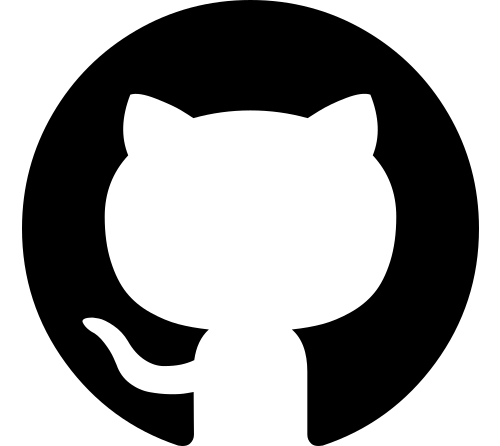
\includegraphics[height=.05\textheight]{resources/github-icon.png}}
  
\includegraphics[height=.05\textheight]{resources/slack-icon.png} ComicSansMS /
  \href{https://twitter.com/DerGhulbus/}{
\includegraphics[height=.05\textheight]{resources/twitter-icon.png} @DerGhulbus}

\end{frame}


\end{document}
